\chapter{Методики повышения эффективности поиска ЛВ}
\label{part:two}

В этой главе рассматриваются задачи построения эффекивных структур данных для представления выражений языка ПО--формул, задача адаптации существующих алгоритмов, используемых в различных системах АДТ для повышения производительности процесса поиска ЛВ, а также разработка других специализированных алгоритмов. Задача этой главы --- реализовать полезные свойства ПО--исчисления при помощи известных и оригинальных продуктивных методик поддержки различных этапов эффективного построения ЛВ. В качестве таких методик и алгоритмов выбраны: разделение данных (data sharing) \cite{Che2, Ryazanov2003}; индексирование данных (term indexing) \cite{HARIndex, TermIndexingBook,pathindex}; параллельные стратегии; для эффективной работы с предикатом равенства использованы результаты теории систем переписывания термов \cite{Nipkow}; Предложен ряд стратегий работы с неограниченными переменными; обобщена и расширена стратегия $k$--опровержения \cite{ICDS2000, dissChe} до стратегии $k,m$--ограничения; разработана структура данных --- дерево состояний вывода, позволяющая реализовать одновременно некоторые из перечисленных методик, один из подходов к разделению данных и процедуру возврата (backtracking). Кроме того реализован ряд других эвристик для поиска ЛВ.


%===================================================================
%===================базовые структуры данных========================
%===================================================================
\section{Структуры данных}

%\app{Это реализация или алгоритмы, причем тут типы? Алгоритм+Стр. данных = Программа (Вирт))}

\paragraph{Тегирование структур данных.}
В основе представления термов и атомов в системе лежит структура \texttt{Symbol}. % или как там она...
Для дифференциации термов в этой структуре данных используются следующие теги: \texttt{ATOM} (атомарный символ), \texttt{FUNCTION} (функциональный символ), \texttt{CONSTANT} (константный символ), \linebreak \texttt{AVARIABLE} (универсальная переменная), \texttt{EVARIABLE} (экзистенциальная переменная), \texttt{UHE} (неопределённый эрбранов элемент (НЭЭ), о нём более подробно рассказано ниже, в разделе про неограниченные переменные), \texttt{INTEGER} (целочисленный символ), \texttt{STRING} (строковый символ). Данные значения теговых полей структур определяются перечислением:

{\tt enum SymbolType \{CONSTANT, EVARIABLE, AVARIABLE, FUNCTION, ATOM, INTEGER, STRING, UHE\};}

\paragraph{Символ (\texttt{Symbol}).}
Символ -- это идентификатор, используемый при построении терма. Структура \texttt{Symbol} содержит:
\begin{enumerate}
\item Строковое представление символа. Необходимо для удобного (читаемого) вывода термов, а значит и формул, на экран.
\item Тегирование символа, одним из перечисленных выше тегов.
\item Арность. Числовое значение, указывающее на количество аргументов, допустимое для данного символа. Для констант, переменных, числовых символов и строк, значение равно нулю.
\end{enumerate}

Символ идентифицируется его адресом в оперативной памяти ЭВМ. Это значит, что два символа, хотя и могут иметь одинаковое строковое представление, но тем не менее будут разными символами. В основном это касается переменных, управляемых разными кванторами, но имеющих одинаковое строковое представление.

\paragraph{Обобщённый терм (\texttt{GTerm}).}
Название для структуры взято из \cite{NNN}. Данная рекурсивная структура данных используется как для представления термов, так и для представления атомов, в виде деревьев.

Разные термы требуют соответствующих способов их обработки. Например, вместо универсальной переменной, возможно подставить другой терм, тем самым конкретизировав её, вывод на экран конкретизированной и неконкретизированной переменной отличается; обработка  структур, представляющих функции, требует учёта наличия и количества аргументов; вместо НЭЭ не может быть подставлена универсальная переменная; и пр. Поэтому способ работы с термом зависит от символа, лежащего в корне дерева, представляющего данный терм. Символ несёт необходимую информацию, в том числе тег. Структура символа определяет в терме необходимое количество памяти под аргументы или возможные конкретизации (подстановки).

Обобщенный терм представляется классической рекурсивной древовидной структурой, каждый узел которой содержит экземпляр структуры \texttt{Symbol} и массив ссылок на его аргументы. Универсальная переменная (\texttt{AVARIABLE}) и неопределённый эрбранов элемент (\texttt{UHE}) не содержат дочерних узлов, но используют единственный элемент одноэлементного массива ссылок-ар\-гу\-мен\-тов как ссылку на терм, который конкретизирует термы с тегом \texttt{AVARIABLE} и \texttt{UHE}. При помощи этой ссылки реализуется конкретизация (подстановка). Если эта ссылка не является \texttt{NULL}, то значит соответствующая переменная (или НЭЭ) конкретизирована некоторым термом, на который указывает ссылка. В противном случае переменная (или НЭЭ) является свободной для подстановки (неконкретизированной). Если переменная (или НЭЭ) конкретизирована, то терм представляющий (тегированный) переменную (или НЭЭ) в данный момент представляет конкретизирующий терм. При этом глубина конкретизации может быть сколько угодно большой, например, при такой подстановке ${\theta}_d = \{x \rightarrow h_1, h_1 \rightarrow h_2, h_2 \rightarrow e \}$, где $x$ --- универсальная переменная, $h_1, h_2$ это НЭЭ, а $e$ --- константа, после применения ${\theta}_d$, переменная $x$ фактически конкретизирована до константы $e$, и дальнейшая работа с термом $x$ производится как с константой $e$ (в том числе вывод на экран). Для корректной работы с конкретизациям реализован метод {\tt GTerm get\_value()}, который возвращает самую глубокую конкретизацию данного терма. Если заданный терм $t$ не является переменной (или НЭЭ) или, в противном случае, если переменная (или НЭЭ) неконкретизирована, то значение \texttt{GTerm get\_value()} совпадает со ссылкой на $t$. Иначе возвращается ссылка на самый глубокий терм, которым конкретизирована переменная (или НЭЭ).

Описанный выше подход к конкретизации термов необходим для того, чтобы корректно и эффективно производить откат подстановок, а для этого необходимо сохранять информацию о том, какая переменная (или НЭЭ) была конкретизирована, и каким значением/термом. Для того, чтобы распознать конкретизацию достаточно проверить первый аргумент массива аргументов на совпадение с \texttt{NULL}, а для того, чтобы откатить подстановку, значению аргумента просто присваивается \texttt{NULL}.

\paragraph{Подстановка \texttt{Answer}.} Подстановка есть список связей (\texttt{Binding}) вида $X \rightarrow t$. В структуре \texttt{Binding} для $X$ и $t$ заданы имена \texttt{left} и \texttt{right} соответственно. По сути \texttt{Binding} есть простая подстановка для одного терма. Как для \texttt{Answer} так и для \texttt{Binding} определены следующие методы:
\begin{itemize}
\item{\texttt{apply()}} --- применить подстановку. В каждой связи терм \texttt{left} конкретизируется до терма \texttt{right}, т.е. аргумент \texttt{left} ссылается на \texttt{right}.
\item{\texttt{reset()}} --- сброс подстановки. Аргумент \texttt{left} являющийся переменной приводится в состояние \texttt{NULL}, а \texttt{left} являющийся НЭЭ не сбрасывается. Применяется непосредственно после шага вывода, для того чтобы освободить переменные для дальнейшего использования, но при этом сохранить НЭЭ конкретизированными.
\item{\texttt{full\_reset()}} --- сброс всей подстановки, включая НЭЭ. Применяется на этапе неудачной унификации, чтобы вернуть все НЭЭ в прежнее состояние.
\end{itemize}

Отметим, что реализация системы задана таким образом, что изменения термов в подстановке, ведут изменения термов во всей формуле. Все изменения термов в формуле выполняются через подстановки.

%----------------------ЧАНК-------------------------------
\paragraph{Чанк} --- это односвязный список элементов типа {\tt T}, в котором выделен его первый ({\tt first}) и последний ({\tt last}) элементы. При помощи чанков организуется основное хранение информации о ПО--формулах и состоянии ЛВ. Чанк называется пустым, если он не содержит элементов, при этом \texttt{first} и \texttt{last} принимают значения NULL. Будем говорить что чанк $C_1$ связан с чанком $C_2$ слева, если узел last чанка $C_1$ ссылается на узел first чанка $C_2$, при этом $C_2$ связан с $C_1$ справа. Для связи чанков определена процедура связывания {\tt void link(Chunk!(T) c)}, которая связывает слева текущий чанк и чанк {\tt c}. Если чанки не пусты, то связывание производится согласно определению. Если один из чанков пуст, то при связывании его элементам \texttt{first} и \texttt{last} присваивается значение того элемента с которым он связывается. Отметим, что несколько чанков могут быть одновременно связаны с другим чанком с одной его стороны. Таким образом процедурой связывания можно построить дерево чанков, растущее от листьев.

На рисунке \ref{fig:chank1} представлен пример структуры, образованной чанками.
\begin{figure}[h]
	%\vspace{0.5cm}
	\centering
	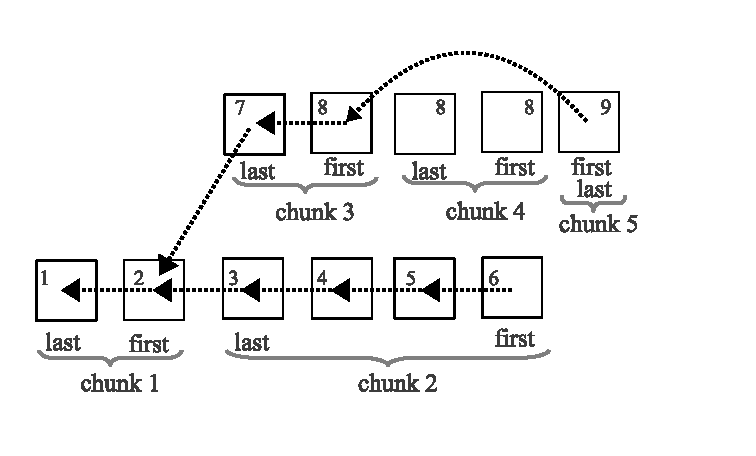
\includegraphics[width=0.8\linewidth]{pics/ChunkFull.eps}
	\caption{Чанки}
	\label{fig:chank1}
\end{figure}
Здесь изображено пять чанков. Друг с другом связаны через поле \texttt{first} следующие чанки: 5 и 4, 4 и 3, 3 и 1, 2 и 1. Чанк 4 является пустым. \texttt{first}  и \texttt{last} это первый и последний узлы чанков. Числа обозначают идентификатор узла. Отсюда видно что пустой чанк дублирует узел \texttt{first}. связанного слева с ним чанка.

Поясним смысл данной структуры. В отдельный чанк заносится информация о состоянии текущего шага логического вывода, поскольку информация разнородна, то для каждого конкретного случая тип {\tt T} конкретизируется. Связанные чанки образуют совокупность информации о шагах логического вывода. Данная структура, хотя и является довольно простой, тем не менее, позволяет реализовать и совместить многие предложенные в работе подходы.



%===================================================================
%=================== ДЕРЕВО СОСТОЯНИЙ ВЫВОДА =======================
%===================================================================
\subsection{Дерево состояний вывода}
Одним из основополагающих средств реализации поиска ЛВ в разработанной системе АДТ является \emph{дерево состояний вывода} (ДСВ), которое строится, в основном, при помощи структур данных, базирующихся на чанках. В структурах ДСВ, с одной стороны, хранится вся совокупность шагов вывода, по которой можно распознать какие действия были произведены на каком шаге, с другой стороны, ДСВ представляет текущую опровергаемую формулу. Основная задача ДСВ заключается в том, чтобы строго зафиксировать все события, произошедшие на каждом шаге логического вывода. Примером фиксируемого события является факт применения подстановки в базовой подформуле к некоторому вопросу. Такая фиксация событий позволяет:
\begin{enumerate}
 \item Использовать больше информации о выполненных действиях, тем самым анализировать процесс ЛВ, а значит эффективно (в смысле большего разнообразия вариантов управления) внедрять эвристики в базовую стратегию поиска ЛВ.
 \item Производить поиск ЛВ с возвратом (backtracking) в процессе построения ЛВ.
 \item Реализовать стратегию разделения данных (data sharing) для случая расщепления базовых подформул после ответа на вопрос с дизъюнктивным ветвлением.
 \item Производить эффективное (в смысле удобства реализации системы АДТ и производительности) управление оперативной памятью.
\end{enumerate}

Идея использования ДСВ базируется на анализе свойств исчисления ПО--формул, проявляемых в процессе построения ЛВ. После каждого ответа на вопрос к первоначальной базовой подформуле добавляется пример консеквента этого вопроса: в базу добавляются соответствующие элементы узлов, непосредственно следующих за вопросом; к списку вопросов базы, в общем случае, добавляются новые вопросы; в случае дизъюнктивного ветвления база расщепляется. Таким образом, формула монотонно увеличивается, при этом сохраняя свою эвристическую структуру. ДСВ используется для обеспечения полного доступа к информации о текущем и прошлом состоянии поиска ЛВ формулы, а также для обеспечения возможности отката поиска ЛВ (backtracking) и подробного наблюдения (сбора статистики) за процессом поиска ЛВ.

Более детально, \emph{дерево состояний вывода} есть такое дерево, которое обладает следующими свойствами: корень дерева есть одна из базовых подформул исходной ПО--формулы; все остальные узлы есть добавляемые консеквенты с применёнными к ним подстановками--ответами с необходимым разыменованием переменных. Если приводить в пример определение \ref{omega} из Главы~1 правила вывода, то корень дерева --- это база $B(\Phi)$, а узлы --- это $C_i(\Psi_i)\theta$. Таким образом, если происходит расщепление базы то в соответствующем узле ДСВ появляется ветвление. Теперь можно говорить, что каждая базовая подформула в формуле характеризуется соответствующим путём от листа ДСВ до её корня.

Как видно, каждый узел содержит достаточную информацию и для того, чтобы производить откат поиска, для этого достаточно просто удалять соответствующие узлы. Кроме того, такой подход реализует разделение данных (ссылок) на каждый консеквент, поскольку некоторые пути могут иметь общие подпути. Если какая-то база опровергнута, то можно удалить все узлы от соответствующего листа до ближайшей точки ветвления, поскольку оставшаяся часть пути всё ещё используется для представления других баз. Количество листовых узлов ДСВ равно текущему количеству баз. Если дерево пусто, значит первоначальная база опровергнута. Так как изначальная формализация задачи в языке ПО--формул может содержать несколько базовых подформул, то для каждой из этих базовых подформул строится своё ДСВ.

Для практических нужд разработки специализированных версий системы АДТ узел ДСВ позволяет сохранять некоторую системную информацию:
\begin{enumerate}
\item Множество атомов--фактов, добавленных к базе на данном шаге вывода (который характеризуется узлом ДСВ). Данное множество представляется как чанк. Отсюда каждый базовый конъюнкт на данном шаге вывода характеризуется объединением всех чанков от данного узла до корня, при этом чанки являются связанными.
\item Список ссылок на вопросы к базе, добавленные на данном шаге вывода. Как и в случае с базовым конъюнктом, вопросы представляются связанными чанками.
\item Для каждого вопроса хранится чанк соответствующих ответов на данном шаге вывода.
\item Номер последующего шага вывода и соответствующий ответ, если узел имеет потомков.
\item Чанк использованных ответов.
\item Индексные множества (подробнее ниже в разделе про индексирование термов).
\end{enumerate}
Кроме того, узлы ДСВ содержат разнородную информацию, используемую как параметры к стратегиям поиска логического вывода.

При помощи чанков получается разграничивать данные, полученные на каждом шаге, т.е. всегда возможно определить какие данные на каком шаге выводы были добавлены, и какие события произошли. Под данными имеются ввиду: атомы--факты, вопросы, ответы и т.п. С другой стороны, на каждом шаге (в каждом узле) доступны все собранные до этого данные.

ДСВ для формулы из примера \ref{proofexample} Главы~1 представлено на рис.~\ref{fig:pst}. Стрелками обозначены не связи узлов--чанков, а направление поиска ЛВ и соответственно роста ДСВ. Корнем ДСВ является исходная ПО--формула $F_1$. Узел 2 является консеквентом вопроса $Q_1$, а именно $\exists\colon A(a)$, а путь от узла 2 до корня соответствует ПО--формуле $F_2$. Узлы 3 и 4 соответствуют консеквентам вопроса $Q_4$. Путь от узла 3 до корня и путь от узла 4 до корня соответствуют базовым подформулам ПО--формулы $F_3$. Например, формулы определённые путями 5---1 и 3---1 разделяют данные, которые представлены узлами 1---2. Если базовая подформула, которая представлена узлами пути 3---1 опровергнута, то можно удалить путь от узла 3 до ближайшего ветвления (в сторону корня), в данном случае удаляется только узел 3, поскольку узлы 2---1 всё ещё используются для представления других базовых подформул.
\begin{figure}[h]
	%\vspace{0.5cm}
	\centering
	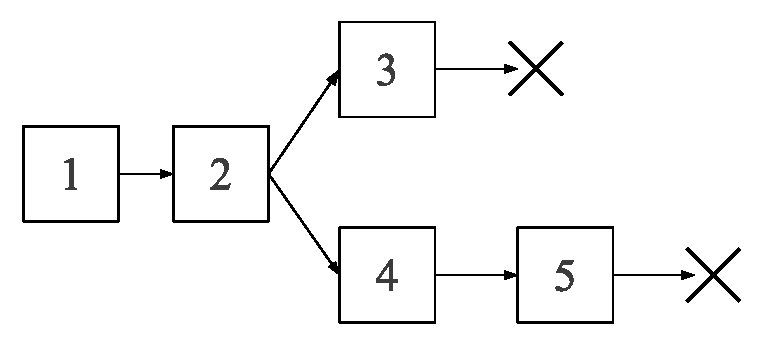
\includegraphics[width=0.4\linewidth]{pics/PST.eps}
	\caption{Дерево состояний вывода для формулы из примера \ref{proofexample}}
	\label{fig:pst}
\end{figure}
На рис.~\ref{fig:pst2} представлено ДСВ из рис.~\ref{fig:pst}, как связанные чанки.
\begin{figure}[h]
	%\vspace{0.5cm}
	\centering
	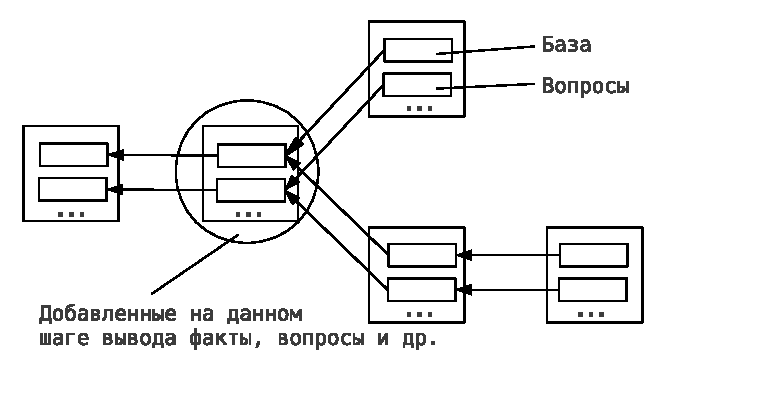
\includegraphics[width=0.7\linewidth]{pics/PST2.eps}
	\caption{Дерево состояний вывода рис.~\ref{fig:pst}, представленное в виде чанков}
	\label{fig:pst2}
\end{figure}

Специфика связывания чанков, характеризует ДСВ как дерево направленное от листьев к корню.
%\rem{С точки зрения реализации ДСВ растёт от листов к корню}{Не понял. Причем тут реализация? \app{М.б. это просто свойство структуры, как, например, в Linux директорий /var всегда растет.}}.

Для ДСВ реализована процедура редукции {\tt merge()}, преобразующая цепь узлов ДСВ в один узел. Это позволяет сократить используемую память, за счёт утраты подробной информации о шагах вывода, соответствующих цепочке узлов ДСВ.




%============================================================================
%================================== РАЗДЕЛЕНИЕ ДАННЫХ =======================
%============================================================================
\section{Стратегии экономии памяти}
Логический вывод практически всегда связан с получением новой дополнительной информации, ростом объема используемой оперативной памяти. Например, в методе резолюции выводятся (синтезируются) новые дизъюнкты до тех пор пока не получится пустой дизъюнкт, а в методе доказательства ПО--формул производится насыщение баз фактами до тех пор, пока все базы не станут содержать противоречие. Поскольку сложность формул может быть сколько угодно большой и даже минимальный вывод может иметь сколько угодно большую длину, имеет место проблема исчерпания имеющихся ресурсов вычислительной системы на хранение разрастающиеся структуры формулы. Опыт показывает \cite{TermIndexingBook}, что автоматический вывод довольно быстро занимает всю имеющуюся в распоряжении оперативную память, и далее процесс вывода требует регулярное удаление излишков. За излишки можно принять любые части формулы. Например, в некоторых системах, основанных на методе резолюций, удаляются дизъюнкты, которые либо вообще не участвовали в выводе, либо не участвовали в нём определённое количество шагов, иногда удаётся определить, что дизъюнкт больше не пригодится, либо предположить, что не будет использоваться и возможно потерять полноту вывода. В случае ПО--формул, излишками являются устаревшие факты, фиктивные вопросы. Таким образом, проблема экономии оперативной памяти является основной проблемой, решаемой в диссертации, особенно с учётом увеличения сложности задач.

Для экономии памяти используются, во-первых, проектирование компактных структур данных; во-вторых, методы разделения общих участков оперативной памяти (data sharing). В случае логических языков и конкретно языка ПО--формул использование методик хранения информации с разделением общей памяти является продуктивным: экономия памяти позволяет строить как более глубокие, так и более широкие ЛВ. Исходя из некоторых общих особенностей представления языков первого порядка и представления ПО--формул, выделено и реализован ряд методик разделения данных.


\paragraph{Агрессивное разделение термов.} Данная методика заключается в том, что разделяются общие участки оперативной памяти среди термов. Например, в термах $A(g(a,f(x)),h(c))$ и $B(k,g(a,f(x)))$, подтермы $g(a,f(x))$ являются общими и представляют собой один и тот же участок в памяти. Данный подход позволяет экономить большие объемы оперативной памяти при ограниченных ресурсах, однако требует дополнительное процессорное время на вычисление общих подтермов. Каждый новый созданный терм (например, факт, добавляемый в базу) проверяется на наличие в нём подтермов, уже используемых где-либо, т.е. производится полный поиск подтермов по базе. Если подтерм найден, то для него переносится ссылка на уже существующий. Такой метод является общеупотребимым в системах АДТ, некоторые варианты реализации представлены в \cite{Ryazanov2003}.

\paragraph{Мягкое разделение термов.} отличается от агрессивного подхода намного меньшим потреблением процессорных ресурсов, но и меньшей эффективностью с точки зрения объема экономии памяти, поскольку разделяет только часть общих подтермов. Исходя из определения \ref{ircond} Главы~1, применение правила вывода $\omega$ корректно в случае выполнения условия $A\theta \subseteq B$, где $A$ и $B$, соответственно, конъюнкты вопроса и базы. Поскольку $B$ это уже существующее множество основных обобщенных термов, то для их хранения выделена соответствующая оперативная память. Подстановка $\theta$ же является отображением переменных вопроса $A$ в элементы эрбранова универсума. В дальнейшем при выполнении шага вывода $\theta$ применяется (апплицируется) ко всему консеквенту вопроса, и данный консеквент добавляется к формуле. Однако правая часть подстановки уже имеется в оперативной памяти в силу того, что основана она на термах из $B$. Исходя из этого, достаточно использовать ссылки на структуры и уже имеющуюся память, используемые для правых частей подстановки, в тех частях консеквента, где эта подстановка применяется.

Рассмотрим следующий фрагмент базовой ПО--формулы:

$$ \exists A(f(e,g(t)))\colon \forall_x A(f(e,x))\colon \exists B(h(x),x) $$

В данном случае вопрос $\forall_x\colon A(f(e,x))$ имеет ответ $\theta = \{x \rightarrow g(t)\}$. К базе фактов добавляется $B(h(x),x)\theta$, т.е. $B(h(g(t)),g(t))$. На рис.~\ref{fig:datasharing1} представлен пример, демонстрирующий данную ситуацию с точки зрения мягкого разделения памяти.
\begin{figure}[h]
	%\vspace{0.5cm}
	\centering
	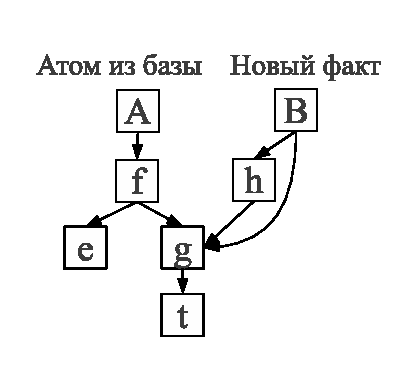
\includegraphics[width=0.3\linewidth]{pics/DataSharing1.eps}
	\caption{Мягкое разделение памяти термов}
	\label{fig:datasharing1}
\end{figure}

%------------Разделение по Черкашину------------
\paragraph{Разделение базовых подформул.} ПО--формулы, в которых производится ответ на вопрос с дизъюнктивным ветвлением, расщепляются на несколько новых базовых подформул. Количество новых базовых подформул совпадает с количеством непосредственных дизъюнктивных подформул в консеквенте вопроса. В простом варианте реализации ЛВ \cite{dissChe} такое расщепление требует копирования предыдущего состояния формулы несколько раз; такое копирование хотя и имеет линейную сложность \cite{Che2}, но всё равно естественно приводит к большим затратам памяти и процессорного времени, затрачиваемого для копирования. Разделение базовых подформул вполне реализуемо при помощи агрессивного разделения оперативной памяти термами. Однако, если формула предполагает достаточно сильное ветвление, сохраняется проблема наличия множества ссылок на разделяемые атомы баз, поскольку конъюнкт представляется как множество ссылок на атомы. Поскольку расщепление предполагает разделение общих частей баз, то имеет смысл разделять упомянутые выше ссылки. Данная стратегия реализуется за счёт средств ДСВ. Любая общая подветвь двух ветвей ДСВ является разделяемой. Рассмотрим небольшой пример. Пусть имеется следующая базовая подформула:
$$\exists A(a)\colon \forall_x A(x)\colon \left\{
\begin{array}{lcl}
 \exists B(x)\colon \forall_y B(y)\\
 \exists C(x)\colon \forall_y C(y)
\end{array}
\right. $$
%Обозначим первый и второй вопросы через $Q_1$ и $Q_2$ соответственно.
Отметим, что данная формула имеет дизъюнктивное ветвление и является глубокой. Из этого следует что в соответствующем ДСВ появится ветвление, а добавленные узлы содержат не только новые факты, но и новые вопросы (в данном случае целевые). ДСВ для опровержения данной базовой подформулы представлено на рис.~\ref{fig:datasharing2}.
\begin{figure}[h]
	%\vspace{0.5cm}
	\centering
	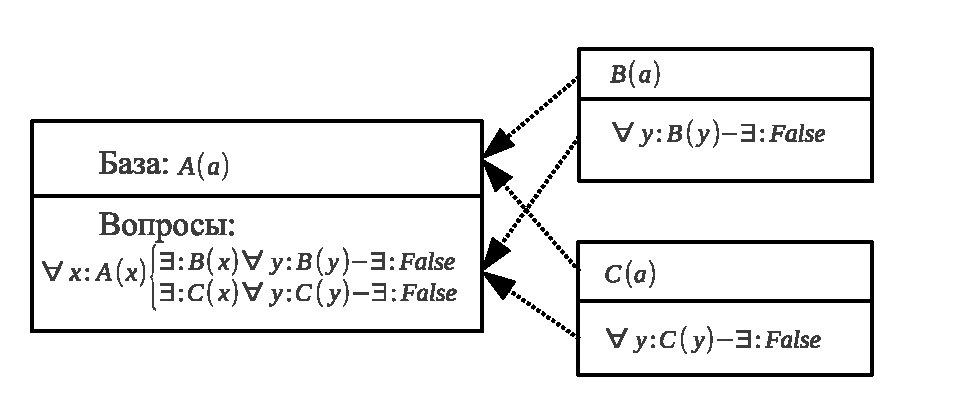
\includegraphics[width=0.82\linewidth]{pics/DataSharing2.eps}
	\caption{Пример дерева состояний вывода опровержения базовой подформулы}
	\label{fig:datasharing2}
\end{figure}

\paragraph{Разделение переменных и НЭЭ.} Данная методика предназначена для высокопроизводительного применения подстановки ко всей подформуле, т.к. все одноименные переменные в формуле представляют собой один участок в оперативной памяти. О неопределенных эрбрановых элементах сказано ниже. Все одноименные переменные на протяжении любого основного пути формулы \cite{dissChe} являются указателем на один и тот же участок в памяти. В отличие от агрессивного разделения данный подход учитывает роль переменных в процессе поиска ответных подстановок. В процессе применения подстановки переменная не заменяется на терм, а лишь указывает на этот терм, что позволяет экономить время на замену переменной термом в поддереве: достаточно одной операции присвоения над одной переменной, чтобы установить замену всех таких переменных в поддереве.


\paragraph{Удаление неиспользуемых фактов.} Ниже, показано что процедура поиска ответных подстановок основана на том, что для каждого атома из конъюнктов вопросов производится попытка унификации с каждым атомом--фактом из базы. Поскольку, количество вопросов и длина конъюнктов конечны, то нетрудно определить для атома--факта из базы, унифицируется ли он хотя бы потенциально с каким-либо атомом из вопросов. Если нет, то такой атом--факт можно удалить из базы, поскольку он вообще не используется в поиске ответных подстановок. Удаление ненужных фактов так же позволяет экономить память и время на переборе фактов. Особенно данная стратегия полезна при исчерпании лимита памяти, поскольку удаление фактов приводит к освобождению памяти.

\paragraph{Веса подформул.} Под весом терма или подформулы понимается количество узлов в дереве, представляющем терм или подформулу. Анализ веса позволяет сдерживать разрастание формулы, и, соответственно, обеспечить дополнительную экономию потребляемой памяти. Для этого из возможных ответов на вопрос приоритет отдаётся тому, который приводит к формуле наименьшего веса. Под весом понимается общее количество узлов в древовидном представлении выражений. Приведем пример, пусть дана следующая простая базовая подформула с одним вопросом:

$$\exists A(t), A(f(e,t))\colon \forall_x A(x)\colon \exists B(x)$$

В данном случае, вопрос имеет два ответа: $\theta_1 = \{x \rightarrow t\}$  и $\theta_2 = \{x \rightarrow f(e,t)\}$. В случае применения ответа $\theta_1$ к базе добавится факт $B(t)$, а в случае применения ответа $\theta_2$ к базе добавится факт $B(f(e,t))$. Предложенная стратегия задаёт приоритет ответу $\theta_1$, поскольку факт $B(t)$ является выражением меньшего веса, чем факт $B(f(e,t))$. Вес факта $B(t)=2$, а вес факта $B(f(e,t))=4$.


\paragraph{Повторы атомов и ответов.} Повторное использование одинаковых ответов, и внесение в базу одинаковых фактов запрещено.

%\rem{...}{Что насчет управления комбинациями методик? Откат и вес? Как задавать эти комбинации? ли это уже реализация, наверное.}

%\paragraph{Ограничение ресурсов.} Стратегия ограниченных ресурсов реализована в большинстве современных систем АДТ, в том числе и в Вампире \cite{Ryazanov2003}. В данной системе АДТ подобная стратегия зависит от текущего ДСВ и описывается следующим образом. Ветка ДСВ растет до тех пор, пока не наступит ограничение объема оперативной памяти, разрешенной для использования, либо пока не исчерпается определенное время, либо пока не будет произведено определенное количество шагов вывода. Если наступил предел использования ресурсов, то осуществляется откат назад и выбор других ответов, т.е. используются другие варианты построения дерева.



%============================================================================
%======================== INDEXING ==========================================
%============================================================================
\section{Индексирование данных.} Формализации некоторых задач могут быть довольно обширными, например задача \texttt{ALG214+4} из библиотеки TPTP в языке ПО--формул занимает порядка 10~Мб. Кроме того, даже если изначальная формула не столь велика, после некоторого количества шагов вывода, она может разрастись до достаточно большого размера. Стратегии разделения данных позволяют лишь отсрочить момент переполнения памяти, а так же вместить в имеющуюся память формулу как можно большего размера. Кроме того, запрет использования повторов требует эффективного поиска заданных выражений по формуле.

С другой стороны существуют ситуации, когда необходимо анализировать ПО--формулу на наличие определённых свойств. Такой анализ проводится как в рамках поиска ЛВ, так и отдельно. Например, если для задачи заданна некоторая стратегия вывода, то для осуществления очередного шага вывода выбирается ответ, а значит база и вопрос, соответствующий этой стратегии, т.е. анализируется вся формула, и выбираются удовлетворяющие части формулы стратегии. Кроме того, анализ формул часто требуется после вывода формулы, для сбора статистики и другой информации, позволяющей в дальнейшем разрабатывать новые стратегии, либо извлекать содержательную информацию из ЛВ.

Отсюда необходимо разработать методы, позволяющие в формуле производить эффективный поиск необходимых её элементов (термов, вопросов, ответов). Для решения данной проблемы обратимся к существующему опыту.

%индексирование термов
\paragraph{Индексирование термов.} Основной структурой, используемой для представления формул, является обобщенный терм. Он используется для представления элементов конъюнктов, кванторных переменных, обеих частей подстановок. Поэтому актуальной задачей является эффективный поиск обобщенных термов в формуле по заданным критериям.

В информационных технологиях поиск данных часто разрешается, например, с помощью методов индексирования данных, применяемых широко в реляционных базах данных БД \cite{Ulman}. В нашем случае основной объект индексирования --- это обобщенный терм, который является древовидной структурой, индексирование которой методами, используемыми в  реляционных БД, неэффективно \cite{TermIndexingBook}. Поэтому используются нижеописанные подходы.

Индексирование термов к настоящему времени хорошо исследовано, как в рамках определенных систем АДТ, так и абстрактно. В частности по данной теме существует ряд интересных работ, в том числе \cite{disctree, subtree, pathindex, TermIndexingBook, HARIndex}. Представленные в этих работах методы позволяют эффективно находить в базе термов такие термы, которые удовлетворяют определенным критериям: являются равными данному (query term), являются его примерами, обобщениями (generalization) и унификациями. Для разработанной системы АДТ требуется поиск заданого терма, его основных примеров, его обобщений, и унификаций. С учетом перечисленных требований а также того факта, что как правило, в базе находятся основные термы, в качестве основы методики индексирования выбрано индексирование путями \cite{pathindex,disctree}. Кратко опишем её суть, как она описана в \cite{disctree}.

Для каждого символа входящего в терм составляется список так называемых \emph{путей}. Путь --- это последовательность чередующихся символов и чисел, где число определяет позицию символа среди дочерних узлов \cite{disctree}. Например, атом $A(e,f(f(x,k),y),m)$ представляется в виде путей $A$, $A1e$, $A2f$, $A2f1f$, $A2f1f1x$, $A2f1f2k$, $A2f2y$, $A3m$. То есть каждому символу соответствует путь от корня до этого символа в древовидном представлении обобщенного терма. Подробнее на рис.~\ref{pathfig} Каждый из этих путей содержит указатель на соответствующий терм, т.е. тот терм, для которого строился путь. Сами пути хранятся в отсортированном виде.
\begin{figure}[h]
	%\vspace{0.5cm}
	\centering
	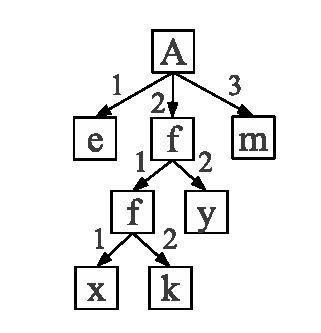
\includegraphics[width=0.25\linewidth]{pics/Path1.eps}
	\caption{Пример построения путей}
	\label{pathfig}
\end{figure}

Пример. Пусть дан атом $A(a,f(x,b))$ и множество атомов
$$\{A(a,f(c,b)), A(a,f(b,e)),A(a,f(k,b)), A(b,f(e,b))\}.$$
Любой атом, являющийся основным примером для заданного, содержит в своём списке путей следующие пути: $A1a$, $A2f2b$. Таким образом, для поиска основных примеров заданного атома необходимо найти пересечение множеств атомов, на которые указывают пути.  В частности путь $A1a$ указывает на множество
$$\{A(a,f(c,b)), A(a,f(b,e)),A(a,f(k,b))\},$$
а путь $A2f2b$ на
$$\{A(a,f(c,b)), A(a,f(k,b)), A(b,f(e,b))\}.$$
Пересечение этих множеств есть множество $\{A(a,f(c,b)),A(a,f(k,b))\}$, это и есть множество примеров для атома $A(a,f(x,b))$.

Методы индексирования термов в настоящее время широко используются во многих известных системах АДТ. %: Vampire -улучшенное индексирование путями, Otter --- дискр.дерево и пути, E, EQP, SPASS --- дерево подстановок.

Отметим следующую особенность внедрения данного подхода к разработанной системе АДТ. Поскольку в системе широко используются методы разделения данных, необходимо совместить индексные множества с подходом к разделению данных. Проблема заключается в следующем. Каждый путь ссылается на множество соответствующих термов, однако поскольку если формула имеет дизъюнктивное ветвление, то в ходе вывода производится её расщепление и ДСВ ветвится соответствующим образом. Для каждой базовой подформулы необходим свой индекс, поскольку базовые подформулы разделяются с использованием возможностей ДСВ, индексное множество также разделяется этой структурой. И вместо списка, традиционно используемого для представления множества термов соответствующих данному пути, строится дерево чанков, в котором множества индексируемых термов соответствуют путям от листа дерева до корня, и каждый такой путь есть индексное множество для данной базовой подформулы. Таким образом, чанковым деревом для хранения индексных множеств может служить ДСВ. Поскольку совмещение метода индексирования путями с методами разделения данных базируется на совмещение индексных множеств с ДСВ, в системе, кроме того, реализуется подход к быстрому откату индекса. Отличие от традиционно используемого метода индексирования путями заключается в том что каждый путь ссылается не надо одно множество соответствующих термов, а на ряд таких множеств, каждое из которых соответствует базовой подформуле, но при этом множства разделяются возможностями ДСВ и тем самым не создают лишней нагрузки на систему (копирование индексных множеств, простые возвраты). Поясним данный подход на следующем примере.
Пусть дан фрагмент базовой подформулы
$$
\exists A(e,k),B(a,b)\colon \forall_x B(x,y) \left\{
\begin{array}{lcl}
 \exists A(x,k) \\
 \exists A(y,k)
\end{array}
\right.
$$

Ответ на вопрос приведет к расщеплению базовой подформулы на две, с конъюнктами $\{A(e,k),B(a,b),A(a,k)\}$ и $\{A(e,k), B(a,b),A(b,k)\}$. ДСВ с указанием разделяемых базовых конъюнктов показано на рис.~\ref{fig:sharedindex}

\begin{figure}[h]
	%\vspace{0.5cm}
	\centering
	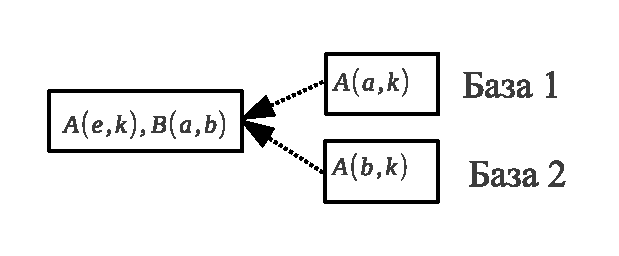
\includegraphics[width=0.6\linewidth]{pics/SharedIndex.eps}
	\caption{Дерево состояний вывода с указанием разделяемых базовых конъюнктов}
	\label{fig:sharedindex}
\end{figure}

На рис.~\ref{fig:sharedindex2} представлен индекс данного множества термов с учетом разделения данных.

\begin{figure}[h]
	%\vspace{0.5cm}
	\centering
	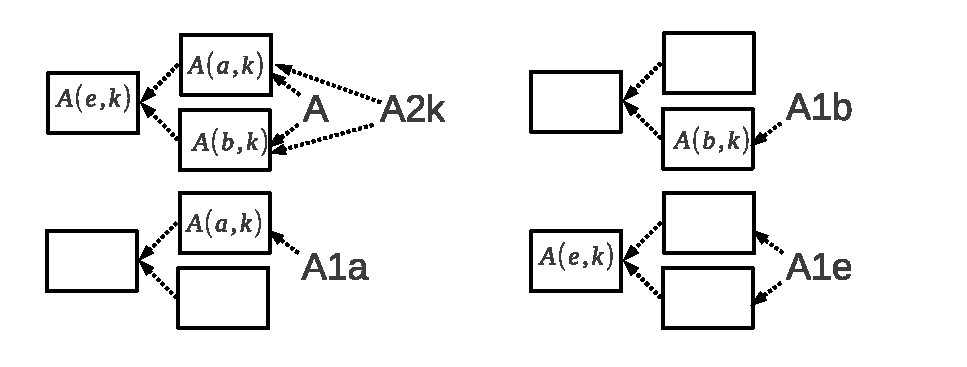
\includegraphics[width=0.82\linewidth]{pics/SharedIndex2.eps}
	\caption{Индексирование путями с учетом дерева состояний вывода}
	\label{fig:sharedindex2}
\end{figure}



%индексирование других частей формулы
\paragraph{Индексирование других частей формулы.} Кроме базы термов, в индексировании нуждаются множества вопросов и множества ответных подстановок. Поскольку количество вопросов не так велико как количество термов, то достаточно использовать возможности обычного словаря.
Теперь опишем другие проблемы, решаемые при помощи методов индексирования данных. Предположим, что пользователем задана некоторая стратегия для решения некоторого класса задач. Стратегия оперирует вопросами с определенными свойствами (т.е. с вопросом сопоставляется содержательная информация), которые присущи всему классу задач (т.е. все задачи объединяет наличие определенных вопросов). Для повышения производительности поиска ЛВ необходимо упростить в дальнейшем доступ к таким вопросам, чтобы каждый раз повторно не проверять все вопросы на наличие определенного свойства. Для этого достаточно сделать словарь (map) в котором каждому описанию вопроса соответствует указатель на данный вопрос. %\rem{В принципе, в стратегиях задавать опции при помощи номеров вопросов, но тогда теряется гибкость: пользователю необходимо ставить вопросы всегда на одно и тоже место. Данный вид индексирования (весьма простого) может выполняться как на этапе компиляции (тогда в компиляции прувера будет задействован не только стратегия но и сама задача), так и при первичном обращении к вопросу (тогда нет необходимости в компилировании самой задачи).}{О чем это?}


\paragraph{Индексирование ПО--формул.} Доказательство крупных формул может производиться в несколько этапов, с сохранением промежуточных результатов на жесткие носители информации. Сам логический вывод формально является цепочкой формул. Для анализа описанных ситуаций необходимо проверять формулы на наличие некоторых свойств. Поскольку, ПО--формула как и обобщенный терм имеет древовидную структуру, то для её индексирования применимы описанные выше методы индексирования путями. Однако в данном случае индексирование путями требует доработки, поскольку, в случае термов путь однозначно задавался символами и номерами дочерних узлов, то в случае ПО--формул номера дочерних узлов сохраняются, а вот символу может соответствовать любая формально описанная характеристика узла ПО--формулы (типового квантора). В системе используются следующие характеристики: тип квантора, размер конъюнкта, лексикографическое представление одного из термов конъюнкта  %[Буду дописывать данный параграф. Есть поле для размышлений. Можно на статью небольшую сделать. В книгах про индексирование подобные задачи описаны как нужные.]



%============================================================================
%================================== ЛЕНИВАЯ КОНКРЕТИЗАЦИЯ =======================
%============================================================================
\section{Неограниченные переменные}
\label{s:uhe}
Проблема неограниченных переменных описана выше. Кратко опишем её суть. Согласно определению \ref{ircond} Главы~1 правило вывода $\omega$ применимо в том случае если вопрос $\forall \bar{y}\colon A$ к базе $\exists \bar{x}\colon B$ имеет {\em ответ} $\theta$  такой что $\theta$ есть подстановка $\bar{y} \rightarrow H^{\infty}$ и $A\theta \subseteq B$. В случае если все переменные из $\bar{y}$ содержатся в конъюнкте $A$, то поиск соответствующих элементов из $H^{\infty}$ производится с помощью алгоритма поглощения и зависит только от сооветствующей базы фактов, поскольку должно выполнятся условия поглощения множеств. Если же среди $\bar{y}$ имеются переменные, которые не входят в $A$, то такие переменные называются \emph{неограниченными} и не используются в алгоритме поглощения. Однако для этих переменных необходимо найти подстановку, причём любой элемент эрбранова универсума является формально корректной подстановкой. Проблема в том, что в общем случае (при наличии функциональных символов) эрбранов универсум является бесконечным множеством, и какой именно элемент из него необходимо выбрать неизвестно.

Данная проблема не является тривиальной. Предложено несколько подходов её решения.

\subsection{Стратегия ленивых конкретизаций}
Суть ленивой конкретизации заключается в следующем. В качестве подстановки для неограниченной переменной выбирается не конкретный элемент эрбранова универсума, а {\em неопределенный эрбранов элемент} (НЭЭ), который, в дальнейшем, исходя из стратегии поиска необходимых термов для построения шага вывода, постепенно конкретизируется до основного терма, либо, в некоторых ситуациях, так и остается неконкретизированным. В данном случае необходимые термы обеспечивают возможность ответа на вопрос: НЭЭ постепенно конкретизируется таким образом, чтобы можно было на очередном шаге вывода построить новый ответ на какой--либо или заданный вопрос. Одновременно решается следующая задача: до какого терма конкретизировать НЭЭ, чтобы появился ответ на вопрос? Отметим, что НЭЭ первоначально появляется как часть ответа в одном вопросе, а его конкретизация производится при поиске ответов на другие вопросы. Под ``постепенной конкретизацией'' понимается процедура ленивых вычислений: НЭЭ конкретизируется настолько точно, насколько этого достаточно для ответа на текущий вопрос, т.е. конкретизация может быть неполной (т.е. не конкретизирующая НЭЭ до основного терма), например НЭЭ $h$ конкретизируется до $f(h_1)$, где $h_1$ новый НЭЭ.

По своей природе НЭЭ схож с неконкретизированной универсальной переменной в том смысле, что он изменяем, т.е. потенциально конкретизируем, однако все такие изменения должны быть направлены только на конкретизацию НЭЭ, т.е. НЭЭ заменяется только на некий терм (возможно тоже содержащий НЭЭ), либо на другой НЭЭ, но не на переменную. Однако, при замене переменной на НЭЭ, НЭЭ обладает всеми свойствами основного терма.

Рассмотрим пример приложения этой техники в процессе построения логического вывода для следующей формулы.
\begin{equation*}
	\forall \emptyset\colon \exists\emptyset
	\left\lbrace
	\begin{array}{l}
		\forall_x\emptyset\colon \exists A(x) \\
		\forall_x A(f(x))\colon \exists B(f(x)) \\
		\forall B(f(a))
	\end{array}\right.
\end{equation*}
На первом шаге вывода получен ответ $\{x \rightarrow h_1\}$ на первый вопрос, $x$ является неограниченной переменной, $h_1$ --- это неопределённый эрбранов элемент (НЭЭ). После первого шага атом $A(h_1)$ добавляется в базу. На втором шаге вывода получен ответ $\{x \rightarrow h_2\}$ на второй вопрос, и $h_1$ конкретизируется до $f(h_2)$, т.е. фактически ответом является подстановка $\{x \rightarrow h_2, h_1 \rightarrow f(h_2)\}$. После второго шага $B(f(h_2))$ добавляется в базу. Наконец, на третьем шаге получен тривиальный ответ на третий вопрос, и $h_2$ конкретизируется до $a$. Таким образом, можно проследить цепочку конкретизации НЭЭ: $\{x \rightarrow h_1\}, \{h_1 \rightarrow f(h_2)\}, \{h_2 \rightarrow a\}$, т.е. без использования НЭЭ, на первый вопрос необходимо было дать ответ $\{x \rightarrow f(a)\}$, прводящий в итоге к успешному опровержению формулы.

В общем случае существуют особые ситуации. Рассмотрим следующий пример.
\begin{example}\label{example:uhe1}
$$\forall \emptyset\colon \exists M(e) \left\{
\begin{array}{lcl}
 \forall_{x,y}M(x)\colon \exists S(y),M(f(x)),T(x) \\
 \forall_x T(x),S(e)\colon \exists Q(x) \\
 \forall_x Q(x),S(f(e))
\end{array}
\right.$$

Данная формула имеет вывод, например такой. Получаем ответ на первый вопрос подстановкой $\{ x\rightarrow e, y\rightarrow e \}$, в результате в базу попадают факты $S(e),M(f(e)),T(e)$; ответ на второй вопрос есть $\{ x \rightarrow e\}$, и в базу попадает $Q(e)$; полученных фактов в базе недостаточно для ответа на целевой вопрос, поэтому вновь отвечаем на первый вопрос, при этом возможно несколько вариантов ответа, но, что важно, переменную $y$ необходимо заменить на $f(e)$. Выберем, например, следующий ответ $\{x \rightarrow e, y \rightarrow f(e) \}$ и в базу попадет факт $S(f(e))$ после чего на целевой вопрос ответ получается. Заметим, что на первый вопрос необходимо обязательно выбирать те подстановки, которые содержат $y \rightarrow e$ и $y \rightarrow f(e)$, они необходимы для ответа на второй и третий вопросы, соответственно. Формула устроена таким образом что первый и второй вопросы всегда имеют новые ответы.

Теперь рассмотрим работу стратегии ленивой конкретизации. Ответ на первый вопрос будет следующего вида $\{ x\rightarrow e, y\rightarrow h_1 \}$, где $h_1$ --- НЭЭ, и в базу попадают следующие факты $S(h_1),M(f(e)),T(e)$. Ответ на второй вопрос --- $\{ x\rightarrow e, h_1\rightarrow e \}$, в котором $h_1$ конкретизируется до $e$, и, соответственно, находящийся в базе факт $S(h_1)$ конкретизируется до $S(e)$. С этого момента начинается выполнение, фактически, циклической операции, поскольку целевой вопрос не имеет ответа: вновь получаем ответ на первый вопрос, и вновь в базу попадает факт $S(h_1)$, который при ответе на второй вопрос вновь конкретизируется до $S(e)$ и т.д. Однако, если пропустить ответ на второй вопрос, то при ответе на целевой, факт $S(h_1)$ конкретизируется до $S(f(e))$ и на этом вывод закончится.
\end{example}


В общем виде проблема заключается в том, что существуют ситуации, когда с формальной точки зрения НЭЭ конкретизируется корректно, но не там где это требуется, например, раньше, чем это необходимо при ответе на другой вопрос. Либо НЭЭ может конкретизироваться там, где это уже не требуется. Из подобных примеров видно, что ленивая конкретизация не всегда может использоваться напрямую. Необходимы дополнительные эвристические средства обеспечения логического вывода, учитывающие описанные только что проблемы.

%------------первый вариант
\paragraph{Ограничение количества конкретизаций (ограничение~1).} Два НЭЭ будем называть \emph{подобными}, если они получены в результате выбора подстановки для одной и той же переменной. Такая ситуация имеет место если на один и тот же вопрос с неограниченными переменными произведено несколько ответов, и для неограниченных переменных все разы в качестве подстановки выступает новый НЭЭ.

Ограничение одинаковых конкретизаций для подобных НЭЭ позволяет исключить ситуации, когда НЭЭ конкретизируется там, где это уже не требуется, и, как следствие, появляется возможность конкретизировать его в другом месте. Для каждого НЭЭ хранится ссылка на переменную, для которой этот НЭЭ был выбран как подстановка. В вопросах каждой неограниченной переменной соответствует набор термов, до которых конкретизировались НЭЭ соответствующие данной переменной. Таким образом, имеется возможность отслеживать сколько раз и как конкретизировался данный НЭЭ. Если лимит конкретизаций исчерпан, то последующие конкретизации запрещены. Выбор конкретного числа, ограничивающего количество конкретизаций, определяется либо пользователем, исходя из его знаний о задаче, либо это число изначально устанавливается равным $1$, и, далее, это число увеличивается в случае неуспешности вывода за определенное количество шагов или времени.

Использование данного подхода позволяет решить пример \ref{example:uhe1} за 5 шагов, если установить единице лимит конкретизаций для переменной $y$ из первого вопроса. Поскольку $h_1$ не будет конкретизироваться до $e$ второй раз, во втором вопросе.

%--------------------ещё вариант
\paragraph{Сохранение выражений, содержащих НЭЭ (ограничение~2).} Представим другой вариант управления стратегией ленивых конкретизаций. Описанный выше вариант конкретизаций НЭЭ, в том числе используемый в примере \ref{example:uhe1}, не сохраняет исходное выражение, содержащийся в котором НЭЭ конкретизируется. Отсюда возникает проблема потери информации. Например, если в примере \ref{example:uhe1} в базу попадает атом $S(h_1)$, то при необходимости конкретизации $h_1$, конкретизация производится не в самом атоме, а порождается новый атом, такой, как если бы был конкретизирован исходный, т.е. в случае рассматриваемого примера, к базе добавляется атом $S(e)$, при этом атом $S(h_1)$ сохраняется. НЭЭ $h_1$ сохранён, а значит, может использоваться в других вопросах.

Содержательно такой подход означает следующее. Можно считать, что для вопроса с открытыми переменными применяется вся совокупность возможных ответов, т.е. с использованием всех элементов эрбранова универсума. Понятно, что это технически нереализуемо из--за бесконечности эрбановского универсума, поэтому и используется техника ленивых вычислений. В идеале предполагается, что за один раз используются все возможные ответы на вопрос, но на самом деле используются только необходимые ответы. Например, если в некоторой формуле содержится вопрос $\forall_x \emptyset\colon \exists A(x)$, и $H^{\infty}= \{a, f(a), f(f(a)), ...\}$, то использование всех возможных ответов разом приводит к попаданию в базу элементов $\{A(a), A(f(a)), A(f(f(a))), ...\}$, которых бесконечно много. Вместо этого множеству ставится в соответствие элемент $A(h)$, где $h$ --- НЭЭ, и в дальнейшем этот элемент порождает необходимые элементы множества $H^{\infty}$.

В данном случае можно заметить сходство со стратегией ленивых конкретизаций, без каких--либо ограничений. Преимущество подхода с сохранением выражений, содержащих НЭЭ, заключается в том, что выражение, содержащее НЭЭ всегда сохраняется, т.е. не может быть утрачено за счёт применения каких-либо подстановок.

Рассмотрим отдельно два случая. Если конкретизируемый НЭЭ содержится в подформуле-вопросе, и если конкретизируемый НЭЭ первоначально появился после ответа на вопрос с дизъюнктивным ветвлением.

В случае с дизъюнктивным ветвлением, вся совокупность ответов на вопрос означает не просто появление бесконечного конъюнкта, а бесконечно множества конъюнктов, поскольку база ещё и расщепляется. Т.е. конкретизация НЭЭ приводит не просто к порождению нового атома в конъюнкте, а к очередному расщеплению формулы, в той точке ЛВ, в которой впервые появился конкретизируемый НЭЭ. Данную точку легко отследить благодаря структуре ДСВ, в которой сохраняются все события произошедшие на каждом шаге вывода. Однако, ветвление целесообразно проводить не в этой точке, а во всех листах дерева, корнящегося из этой точки. Поскольку вставка ветвления в середину вывода потребует копирования для каждого нового узла той части вывода, которая была уже произведена.  На рис.~\ref{lazy21} схематично показано некоторое ДСВ.
\begin{figure}[h]
	%\vspace{0.5cm}
	\centering
	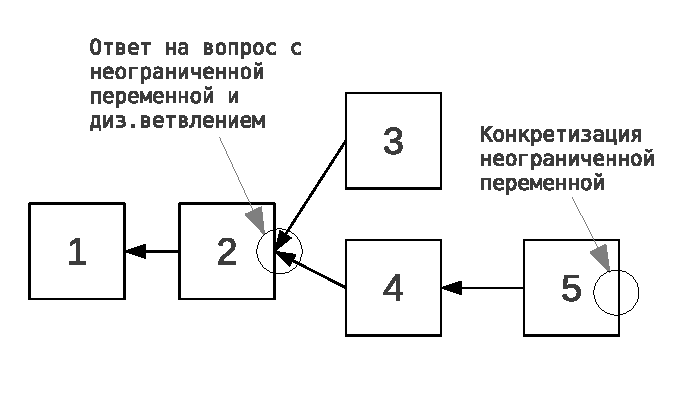
\includegraphics[width=0.5\linewidth]{pics/Lazy21.eps}
	\caption{Структура дерева состояний вывода до конкретизации}
	\label{lazy21}
\end{figure}
После конкретизации НЭЭ, получаем структуру ДСВ, представленное на рис.~\ref{lazy22}

\begin{figure}[h]
	%\vspace{0.5cm}
	\centering
	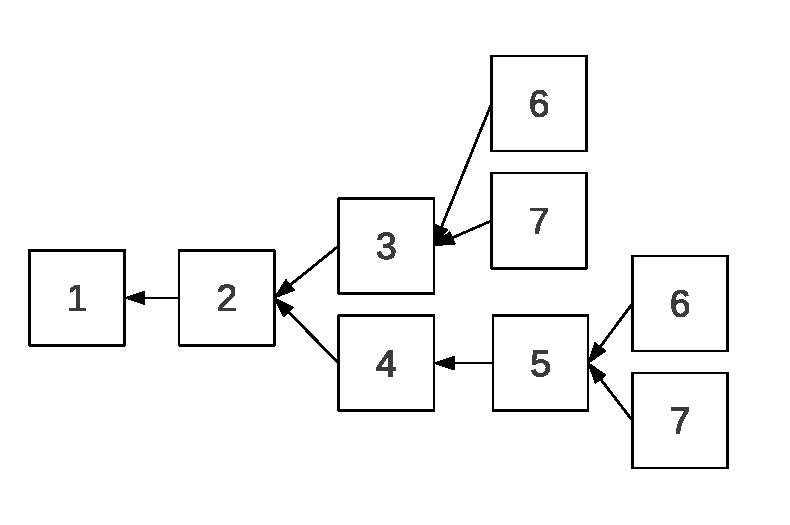
\includegraphics[width=0.5\linewidth]{pics/Lazy22.eps}
	\caption{Структура дерева состояний вывода после конкретизации}
	\label{lazy22}
\end{figure}

В случае подформулы--вопроса, содержащего НЭЭ, конкретизация НЭЭ требует порождения новой подформулы--вопроса, отличающейся от исходной только в точке содержания НЭЭ. Возможно появление множества вопросов, усложняющее в целом структуру формулы и её вывод. Под усложнением структуры, в данном случае, понимается именно наращивание количества вопросов. Абсолютный размер формулы (в байтах) меняется незначительно, поскольку используются стратегии экономии памяти. Новую подформулу--вопрос целесообразно вставлять в той точке вывода (перед этим узлом), где первоначально добавился вопрос с НЭЭ. Предположим что на рис.~\ref{lazy21} вопрос с НЭЭ впервые появляется в узле 2. Тогда если конкретизация НЭЭ потребуется в любом из последующих узлов, дерево преобразуется в вид, как на рис.~\ref{lazy23} При этом новый узел 6 содержит только новый порождённый вопрос.
\begin{figure}[h]
	%\vspace{0.5cm}
	\centering
	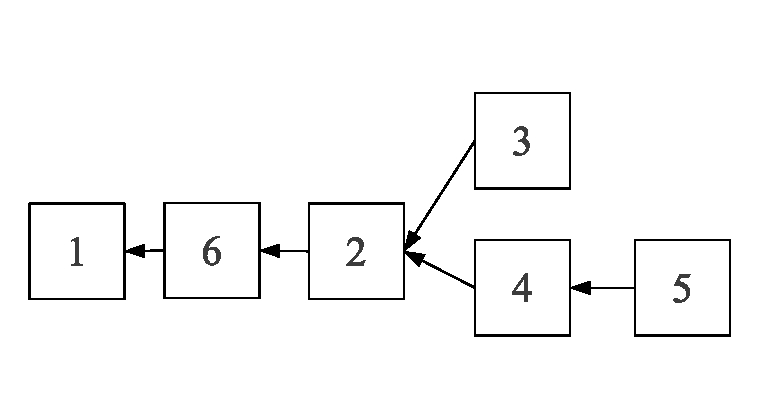
\includegraphics[width=0.5\linewidth]{pics/Lazy23.eps}
	\caption{Дерево состояний вывода после конкретизации в узле без дизъюнктивного ветвления}
	\label{lazy23}
\end{figure}

%---------------второй вариант
\paragraph{Ручное управление.} Одним из вариантов решения проблемы является использование языка описания стратегий, с помощью которого можно, например, указать, что на второй вопрос необходимо ответить лишь один раз, либо использовать на первый вопрос сразу несколько подстановок содержащих $y\rightarrow h_1$ и $y\rightarrow h_2$. Это приведет к попаданию в базу двух фактов $S(h_1)$ и $S(h_2)$, один, из которых будет использоваться для второго вопроса, а другой для целевого. Такой вариант вполне приемлем, и может использоваться для решения задач. Такой подход в настоящее время пока не обеспечивает принципиальную выводимость, но для отдельных классов задач он уместен.

%-------------
Отметим, что стратегии, основанные на использовании НЭЭ, создают некоторые проблемы совместимости с другими стратегиями. Во-первых, при использовании этой стратегии нарушается независимость базовых подформул, поскольку один и тот же НЭЭ может быть в разных подформулах: конкретизация общего НЭЭ в одной подформуле автоматически приводит к конкретизации его в другой подформуле. Этот факт, в частности, делает зависимыми процессы поиска ЛВ в базовых подформулах на параллельных вычислительных архитектурах.

\subsection{Стратегия фильтрации эрбранова универсума}
Другим вариантом (помимо стратегии ленивых конкретизаций) решения проблемы неограниченных переменных, является \emph{стратегия фильтрации эрбранова универсума}. Данная стратегия позволяет избавиться от изложенных в начале главы проблем, но несколько расширяет пространство возможных ответов. Суть данной стратегии заключается в следующем. В консеквентах, атомы которых содержат неограниченные переменные вопросов, должны унифицироваться с одноимёнными атомами из всех других частей всей базовой подформулы, в противном случае атом из консеквента после попадания в базу не будет удовлетворять условию применения правила вывода (Определение~\ref{ircond} Главы~1), поскольку никогда не выполнится процедура унификации при поиске ответов. Будем использовать данное свойство в стратегии. В качестве ответа для неограниченных переменных используются такие термы, что атом полученный подстановкой переменных на эти термы будет основным примером найденной унификации. Такой подход позволяет заранее сузить пространство эрбранова универсума, фильтруя заведомо бесполезные ответы.

Для ясности рассмотрим пример. Пусть имеется следующие вопросы ПО--формулы.
$$Q_1 = \forall_{x,y}\emptyset\colon \exists A(f(x,g(y)))$$
и
$$Q_2 = \forall_x A(f(e,x))$$

В данном случае в консеквенте вопроса $Q_1$ содержится атом $A(f(x,g(y)))$. Одноимённый атом, это атом вопроса $Q_2$, а именно $A(f(e,x))$. Унификация двух данных атомов есть $A(f(e,g(y)))$. Основной пример данного атома есть любой, атом полученный из исходного заменой переменной $y$ на любой элемент $H^{\infty}$. Тогда ответ для вопроса $Q_1 = \{x \rightarrow e, y \rightarrow t\}$, где $t$ любой элемент $H^{\infty}$, например $e$. В базу попадёт факт $A(f(e,g(e)))$ и ответ на целевой вопрос будет $\{x \rightarrow e\}$.

Такой подход имеет сходство со стратегий ленивых конкретизаций, в которой конкретизация НЭЭ, по сути, означает сужение эрбранова универсума, до множества основных примеров конкретизации. В данном же случае ограничения на эрбранов универсум накладываются сразу, исходя из потенциальных вопросов. В случае стратегии ленивой конкретизации, конкретизация как раз производится при поиске ответов на эти потенциальные вопросы.

Данная стратегия позволяет всегда работать с полностью конкретизированной формулой, т.е. формулой не содержащей НЭЭ.




%=============================================================================================
%================================== k,m-ограничение =======================
%=============================================================================================
\section{Стратегия $k,m$--ограничения}
Данная стратегия формулируется следующим образом. Некоторый ответ применяется, если за последующие $k$ шагов произойдет заданное событие, по меньшей мере $m$ раз. Пользуясь терминологией ДСВ, это означает, что для данного узла дерева применяется ответ в случае, если построенное в результате дальнейшего вывода поддерево, коренящееся с этого узла, не превысит глубину $k$, и до этого момента произойдет $m$ раз заданное событие. Данная стратегия хорошо совместима с ДСВ, и использует его возможности для возможных возвратов в выводе. Предложено три специальных случая данной стратегии.

\paragraph{$k,m$--опровержение.} Заданный ответ выбирается в случае, если за последующие $k$ шагов ЛВ будет опровергнуто как минимум $m$ баз. Подобная стратегия, а именно $k$--опровержение, первоначально предложена А.К.~Жерловым в \cite{ICDS2000} и реализована в системе КВАНТ/1 Черкашина Е.А. \cite{dissChe}, где показана её состоятельность. В данной системе эта стратегия расширена вторым параметром $m$. Она позволяет сдерживать разрастание пространства поиска вывода, т.е., сдерживать излишнее ветвление ДСВ, что в некоторых случаях приводит к многократному усложнению вывода.

Отметим, что выбор параметров $k$ и $m$, заранее не определён, и пользователю необходимо знать следующие нюансы. Во-первых, параметр $k$ означает, что будут проверены все возможные ответы на глубине $k$ шагов, т.е. произведен полный перебор, что в свою очередь может затратить большие ресурсы процессорного времени и памяти. Параметр $m$ дополнительно усиливает, условие выбора исходного ответа. Поэтому, если заранее нельзя предположить какие выбрать эти параметры, то по умолчанию они устанавливаются $k=1$ и $m=p$, где $p$ количество непосредственных дочерних дизъюнктивных узлов вопроса, и в случае неудачи ЛВ, параметр $k$ постепенно увеличивается, а $m$ уменьшается. Кроме того, если задать максимально возможное значение $m$, и не использовать других ограничений на полноту вывода, то можно производить полный перебор пространства поиска на глубину $k$.

\paragraph{$k$-неопровержимость.} Для вопроса с дизъюнктивным ветвлением, какой-либо ответ принимается только в случае, если за $k$ шагов не будет достигнуто опровержение базовой подформулы с использованием только вопросов без дизъюнктивного ветвления. Смысл такого подхода, как и в предыдущем варианте, заключается в том, чтобы сдерживать разрастание формулы из-за ответов на вопросы с дизъюнктивным ветвлением. Ответ для такого вопроса применяется только если нет иных (без ветвления) способов опровержения. Отметим, что в данном случае параметр $m$ убран.

\paragraph{$k,m$--конкретизация.} Это разновидность спецификации стратегии $k,m$--ограничения, она формулируется так. Ответ на вопрос принимается, если за последующие $k$ шагов будет конкретизировано $m$ НЭЭ. Эта стратегия также направлена на то, чтобы ограничить сложность представляемой формулы. С неконкретизированным НЭЭ ассоциируется много дополнительной информации и условий, описанных в разделе \ref{s:uhe} о неограниченных переменных, что на уровне реализации влияет негативно. Поэтому чем больше и быстрее НЭЭ будут конкретизированы, тем лучше.



%\paragraph{ стратегии $k,m$--ограничения}
%Основной для реализации данной стратегии являются описанные выше ДСВ. Параметры $k,m$ и, собственно, условие задаются в супервизоре и привязываются к определённому узлу ДСВ. Супервизор проверяет все условия на каждом шаге ЛВ. И в положительном случае (когда условие выполнено) производится возврат поиска (backtracking) назад, т.е. производится последовательное удаление узлов дерева в обратном порядке (от листа в направлении корня). Перед удалением каждого узла производится разконкретизация НЭЭ, полученных в этих узлах и возврат использованных вопросов в стадию активных (т.е. возможных для применения).


%\section{Повторение вывода для исчисления высказывания}


%=============================================================================================
%-----------PARALLEL STRATEGY---------------------------
%=============================================================================================
\section{Параллельные стратегии}

Повышение производительности достигается при помощи вышеописанных интенсивных методов, ориентированных на оптимизацию использования вычислительных ресурсов, а также при помощи экстенсивных методов, базирующихся на вовлечении в процесс дополнительных вычислительных ресурсов. В частности, это становится актуальным ввиду широкого распространения многоядерных вычислительных систем общего назначения, в частности, рабочих станций.

Одним из популярных экстенсивных методов повышения производительности является разработка версий программ АДТ для кластерных архитектур в параллельном режиме исполнения ветвей подпрограмм. Такой подход реализован во многих современных системах АДТ, например в \cite{PSETHEO}.

Рассмотрим методики и стратегии построения параллельных реализаций алгоритмов поиска ЛВ в исчислениях ПО--формул. Предложены следующие стратегии для построения параллельных схем алгоритмов поиска логического вывода.

\paragraph{Первая стратегия: опровержение баз.} В случае, если вопрос имеет дизъюнктивное ветвление, то после ответа на этот вопрос, формула расщепляется и трансформируется в формулу с б\'{о}льшим количеством баз, т.е. в общем случае, количество базовых подформул увеличивается с каждым шагом вывода. С другой стороны, исходная формализация задачи в языке ПО--формул, опять же в общем случае, содержит более одной базовой подформулы. Для того, чтобы показать, что исходная формула противоречива, необходимо опровергнуть каждую из баз. Специфика исчисления ПО--формул позволяет производить логический вывод и опровержение этих баз независимо друг от друга. Данное свойство называется естественным ИЛИ--параллелизмом, который следует из того что в базах находятся лишь основные термы. Поэтому процедура опровержения каждой базы может выполняться в отдельном вычислительном процессе или на отдельном вычислительном устройстве.

Таким образом, первая стратегия, реализуемая в виде параллельной схемы алгоритмов, формулируется следующим образом: каждая базовая подформула, содержащая только основные термы в базе, опровергается независимо от других базовых подформул, а значит этот процесс выделяется в отдельный параллельный независимый от других процесс, синхронизируемый с другими процессами только  на этапах его создания в момент расщепления формулы и завершения в момент установления выводимости/невыводимости. Во время жизни этого процесса к нему может поступать асинхронный сигнал завершения от супервизора, обозначающий, что выполнение процесса далее не имеет смысла, например, формула является неопровержимой, что было доказано в какой-либо другой ветке поиска доказательства, или пользователь остановил выполнение программы. Для программной реализации алгоритмов данной стратегии созданы подпрограммы жесткого копирования и маршаллинга/демаршаллинга, чтобы полностью скопировать базовую подформулу и обрабатывать её в отдельном процессе независимо, т.е. не разделяя оперативную память.

%\rem{...}{Думаю этот раздел немного покажет тебе на сколько подробно можно и надо писать.}

\paragraph{Вторая стратегия: поиск ответов на вопросы.} Для применения каждого шага логического вывода, необходимо выполнять, в общем случае, поиск ответных подстановок для заданного вопроса. Поиск ответных подстановок не изменяет структуру формулы, и не использует общих изменяемых данных, это значит, что процессы поиска ответа на каждый вопрос независимы, а значит параллельны. Отметим, что поиск ответных подстановок для одного вопроса является намного менее трудоёмкой задачей, чем опровержение базовой подформулы, но тем не менее если конъюнкт вопроса содержит достаточно много атомов, то поиск всех ответных подстановок усложняется, за счёт увеличения пространства --- в общем случае декартова произведения множеств подстановок для каждого атома из конъюнкта.

%\rem{...}{М.б. тут тоже рассказать в общих чертах о варианте реализации, например, что это не будет отдельный процесс или узел, а будет поток (нить)}


\paragraph{Третья стратегия: поиск подстановок для атомов вопроса.} Теперь рассмотрим процедуру поиска подстановок для отдельно взятого вопроса. Как было сказано В Главе~1, подстановка $\theta$ является ответом, если выполняется условие $A\theta \subseteq B$, где $B$ --- конъюнкт вопроса, $A$ --- конъюнкт базы. Для сохранения полноты необходимо хотя бы потенциально иметь в распоряжении все возможные ответы, из которых выбирается подстановка для данного шага. Ниже описана структура хранилища ответов. Наполнение каждого чанка хранилища подстановками производится параллельно, поскольку чанки независимы.

\paragraph{Свойства стратегий.} Анализ, описанных выше стратегий, показывает, что они обладают свойством вложенности. Т.е., для того, чтобы опровергнуть одну базовую подформулу (первая стратегия) необходимо найти ответы на вопросы (вторая стратегия). В свою очередь для поиска ответа, необходимо найти подстановки для каждого атома из конъюнкта вопроса (третья стратегия).

Исходя из этого, данные стратегии можно разместить по степени эффективности (иерархия стратегий). Не трудно видеть, что время, затрачиваемое на опровержение базы, как минимум, не меньше, чем время, затрачиваемое на поиск ответных подстановок, а на практике, как правило, оказывается намного больше, так как для опровержения базы необходимо неоднократно ответить на некоторые вопросы. Аналогичные выводы делаются по отношению к другим стратегиям.

Кроме того, можно выделить единое для всех стратегий свойство –-- свойство однородности (стратегии имеют единую структуру). А именно, все они, по сути, сводятся к применению некоторой операции (опровержение базы, поиск ответов и т.д.) для каждого элемента некоторого множества (базы, вопросы и т.д.).

Одной из рекомендаций при реализации описанных алгоритмов на кластерных вычислительных системах является правильное распределение задач между вычислительными узлами кластера, в зависимости от скорости коммуникации между ними. Например, программная реализация первой стратегии должна привязывать процесс к вычислительному узлу. Привязка процесса к вычислительному узлу, в случае второй стратегии, возможна с увеличением конъюнкта вопроса и увеличением множеств подстановок, соответствующих каждому атому вопроса. В противном случае, этого не стоит делать, как и  при реализации третьей стратегии, так как коммуникационные затраты, вполне вероятно, перекроют полезное время вычислений, и тем самым лишь ухудшат результат.

%Отметим что данная стратегия в общем случае конфликтует со стратегией отсроченного присваивания (поскольку СОП может нарушать независимость баз и вопросов). \rem{...}{А это не надо было где-то раньше сказать. Например в разд. ``первая стратегия''?}




%=============================================================================================
%============================= РАВЕНСТВА =========================
%=============================================================================================
\section{Равенства}
Для обработки предиката равенства, как правило, крайне неэффективно напрямую использовать аксиомы равенства (рефлексивность, симметричность, транзитивность, подстановочность) без специальной адаптации алгоритмов АДТ. Например, если формула содержит лишь один бинарный функциональный символ $f$ и один бинарный атомарный символ $A$, то в языке ПО--формул аксиомы равенства для такой формулы будут представлены следующим образом.
$$\left\lbrace
\begin{array}{l}
\forall_x\emptyset\colon \exists x = x \\
\forall_{x_1,y_1,x_2,y_2} x_1 = y_1, x_2 = y_2\colon \exists f(x_1,y_1) = f(x_2, y_2) \\
\forall_{x_1,y_1,x_2,y_2} x_1 = y_1, x_2 = y_2, A(x_1,y_1)\colon \exists A(x_2,y_2)
\end{array}\right.
$$
Как видно, для каждого функционального и атомарного символа из формулы ставится в соответствие подформула--вопрос --- аксиома равенства. Явное использование таких аксиом, во-первых, усложняет структуру формулы (появляются лишние вопросы), во-вторых, значительно увеличивает число шагов вывода, в-третьих, генерирует много (потенциально бесконечно) фактов в базе, возможно не участвующих в выводе, а также мешающих выводу. Отметим, что данная проблема не так ужасна как в МР, поскольку в МР, в общем случае,  порождаются дополнительные дизъюнкты, а это соответствует порождению дополнительных вопросов в ПО--формуле. В исчислении ПО--формул порождаются лишь атомы-факты, за которыми проще наблюдать, в силу их более простой структуры, чем подформулы-вопросы (или дизъюнкты)

Очевидно, что вопросы--аксиомы равенства предназначены для того чтобы выводить те и только те атомы--факты, которые эквивалентны по модулю $E(B)$, другим атомам-фактам из базы $B$. В данном случае $E(B)$ это все равенства из базы $B$.

Для того чтобы не использовать на прямую аксиомы равенства, предлагается генерировать эквивалентные по модулю $E(B)$ атомы--факты с помощью систем переписывания термов (СПТ) \cite{Nipkow}.

Для построения СПТ по равенствам в базе, используется известный алгоритм Кнута--Бендикса (Knuth--Bendix completion procedure) \cite{KBAlg}. Алгоритм Кнута--Бендикса, получая на входе множество атомов--равенств и редуцирующий порядок над термами \cite{Nipkow} строит эквивалентную конвергентную СПТ. Конвергентность СПТ означает, что для каждого терма существует и только одна конечная форма (нормальная форма), которая может быть получена за конечное число переписываний. Под порядком над термами имеется ввиду отношение строгого частичного порядка над множеством термов. В нашем случае используется лексикографический порядок.

С помощью правил переписывания генерируются новые атомы--факты, эквивалентные, уже имеющимся в базе. В сочетании со стратегией удаления неиспользуемых фактов (стратегия экономии памяти), очевидно, что базу не будут добавляться ненужные сгенерированные факты.

Отметим, что такой подход не нарушает основных особенностей исчисления ПО--формул. Правило вывода сохраняется, остаётся единственным и унарным. Ответные подстановки по--прежнему зависят лишь от базы, и не зависят от других вопросов. Базы по--прежнему остаются независимы и содержат основные термы. Структура формулы не изменяется.


\section{Выводы по главе}
Использование представленных в даной главе методик привело к следующим результатам: значительная экономия памяти по сравнению с предыдущими версиями систем АДТ \cite{dissChe}, влекущее за собой экономию вычислительных ресурсов за счёт того, что предотвращается излишнее копирование термов и целых подформул, производится удаление неиспользуемых фактов, и замедляется расзрастание формулы; рост производительности с использованием параллельных стратегий (при условии применимости этих стратегий); сокращение пространства поиска за счет стратегий $k,m$--ограничения, сдерживающих разрастание формулы из--за дизъюнктивного ветвления, и стратегий неограниченных переменных, позволяющих не перебирать эрбранов универсум; за счёт применения методик индексирования термов повышена эффективность доступа к выражениям ПО--формул, и как следствие повышена эффективность поиска ЛВ по времени; эффективный ЛВ с предикатом равенства, по сравнению с явным использованием аксиом равенства.


%В классическом подходе, в соответствии с определением ~\ref{ircond}, подстановка $\theta$ является ответом на вопрос, тогда и только тогда, когда $A \theta \subseteq B$ где $A$ --- конъюнкт вопроса, а $B$ --- конъюнкт базы. Поиск ответов есть задача поглощения, для решения которой, как правило, используется алгоритм мэтчинга \rem{, об этом уже писалось выше}{Это нужно?}. В случае ПО--формул используется основной матчинг, а в случае НЭЭ используется полуосновной матчинг. \rem{...}{Надо прокомментировать где-то ранее эти матчинги, или даже строго определить.}


%Для решения проблемы основного матчинга без явного использования аксиом равенства поставлена задача реализации основного матчинга с равенствами, которая формулируется следующим образом [microsoft]:
%\begin{quote}
%Для данного множества равенств $E(B)$, основного терма $t$ и терма $p$, который может содержать переменные, необходимо найти множество подстановок $\theta$, по модулю $E(B)$, такие что $E(B)\models t = p\theta$. Через $E(B)$ мы обозначим множество всех равенств в данной базе $B$. Две подстановки эквивалентны если их правые части попарно конгруэнты по модулю $E(B)$.
%\end{quote}

%С точки зрения реализации

%Для поиска таких ответов использован аппарат теории систем переписывания термов \cite{Nipkow}.




%%% Local Variables:
%%% mode: latex
%%% TeX-master: "dis"
%%% End:
